\documentclass{article}

\usepackage[utf8]{inputenc}
\usepackage{parskip}
\usepackage{graphicx}
\usepackage{epstopdf}
\usepackage{wrapfig}
\usepackage{mwe}
\usepackage{libertine}
\usepackage{inconsolata}
\usepackage{hyperref}

\newcommand\theversion{0.0.1-git}

\hypersetup{
  hidelinks,
  pdftitle={Pancakes v\theversion},
  pdfauthor={Johann Tutor}
}

\renewcommand{\sectionautorefname}{§}
\renewcommand{\subsectionautorefname}{§}
\renewcommand{\subsubsectionautorefname}{§}
\renewcommand{\paragraphautorefname}{¶}

\setcounter{secnumdepth}{4}

\begin{document}
\title{Pancakes\\ \large A flipping card game, v\theversion}
\author{Johann Tutor}
\date{\today}
\maketitle

Pancakes is a quick and easy-to-learn card game developed by Johann Tutor, originally developed from an ad-hoc session of an Eleusis-like game.

When teaching this game to someone else, it is recommended that they play without being told the rules for the first game;
only answer ``yes''/``no'' questions and correct them when they do something illegal.

\tableofcontents

\newpage

\section{Requirements}

Pancakes uses a standard deck of cards. Jokers are optional but highly recommended.
Up to five players may play.

\section{Setting Up}
\label{sec:setup}

Shuffle the deck. Deal eight cards face-down on the table, then deal one card face-up on each of those to form eight Stacks.
These Stacks should be arranged in four centered rows with 1-3-3-1 Stacks each.
The playing field formed by these eight Stacks is called the ``Griddle''.

Deal five cards to each player and set aside the rest of the deck to be the Draw Pile. Decide on a player order.

\section{Rules}
\label{sec:rules}

The goal of the game is to get rid of all the cards in your hand.

Players take turns placing cards onto Stacks. On each turn, you must place a card on to one of the Stacks, and you may do so in one of two ways: put down a card from your hand, or transfer a card from one Stack to another. If you cannot make a legal play, you must pass. You may only play one card per turn.

\subsection{Playing a Card}
\label{sec:playcard}

You have two ways to play your turn: you may play from your hand, or you may play from the Griddle. Both ways share the same basic rules, differing only in the source of the card to be played.

\subsubsection{Basic Rules}
\label{sec:legalplays}

\paragraph{}
A card may only be placed on an empty Stack or on a Stack whose top card is either the same rank (number), a Joker or a card back.

\paragraph{}
If the card you play is a different color than the one on the top of the Stack, flip the Stack so that the card on the bottom is now on top.

\paragraph{}
Empty Stacks and card backs are always considered the same color as the card played on top unless the card is a Joker.
In other words, playing a card that is not a Joker on top of an empty Stack or a card back does not flip the Stack.

\paragraph{}
Jokers are always considered a different color than the card on which it is played or the card that is played on top of it, including empty Stacks and card backs.
In other words, playing a Joker or playing any card on top of a Joker flips the Stack, even if it is the only card in the Stack.

\subsubsection{Playing From Your Hand}
\label{sec:fromhand}

On your turn, you may choose to play from your hand.

\paragraph{}
If you have a card that you may legally play according to \autoref{sec:legalplays}, play it.

\paragraph{}
If you do not have any cards that you may legally play, draw from the Draw Pile until you draw a card that you may legally play, then play that card.

\paragraph{}
You cannot draw if you have any legal plays in your hand and you must play the first card that gives you a legal play when drawing.
However, if you accidentally started drawing illegally (i.e. you had a legal play in your hand), you must continue to draw until you draw a card that you may legally play. Any cards that would have been legal to play cannot be played until your next turn.

\paragraph{}
If the Draw Pile is or becomes empty while drawing and you still need to draw, you must pass as you have no legal plays.

\paragraph{}
You may not play from the Griddle until your next turn once you have started drawing.

\paragraph{}
If you have no more cards in your hand at the end of your turn, the game ends immediately.

\subsubsection{Playing From the Griddle}
\label{sec:fromstack}

On your turn, you may choose to play from the Griddle instead of your hand. Note that if you have already started drawing, you may not play from the Griddle until your next turn.

\paragraph{}
Take the top card of one Stack and place it on the other Stack. This transfer must be done according to the basic rules outlined in \autoref{sec:legalplays}.

\paragraph{}
If you expose a card back on the first Stack, flip the top card (not the whole Stack) so that it is face-up.

\paragraph{}
Cards may be placed on empty Stacks and card backs, but card backs may not be transferred from one Stack to another.

\paragraph{}
If there are no transfers possible, you must play from your hand. See \autoref{sec:fromhand} for details.

\subsection{Passing}

\paragraph{}
If you choose to play from your hand and you need to draw a card because you have no legal plays, but the Draw Pile is empty, either because it was already empty or because it became empty while drawing, then you must pass as you have no other options.

\paragraph{}
You may not pass if you have a legal play in your hand. Note that it is legal to pass even if there is a legal play on the Griddle as long as the Draw Pile is empty and you have no legal plays in your hand.

\paragraph{}
If everyone passes in succession, shout ``Pancakes!'' and flip all Stacks. If everyone passes immediately after that, the game ends. Note that the game does not end if at least one person can go; in this case, the next time everyone passes, the Stacks are flipped again according to this rule.

\subsection{Winning}

The player who empties their hand first wins the game. If the game ends with everyone passing, the player with the least number of cards in their hand wins the game; if there are multiple players with the least number of cards, they tie.

\subsection{Miscellaneous}

Card counts are public. You may ask another player how many cards are in their hand at any time and they must show you how many cards they have.

\pagebreak
\section{Scoring}

Points are awarded to the winner of the game. The winner's score is calculated as follows: count the number of cards that the other players have, subtract the number of cards the winner has, divide that difference by one less than the number of players, and round up to the nearest whole number.

For the mathematically inclined:

$$
\langle\textrm{Score}\rangle = \left\lceil\frac{\langle\textrm{others'\ cards}\rangle - \langle\textrm{winner's\ cards}\rangle}{\langle\textrm{\#\ of\ players}\rangle - 1}\right\rceil
$$

In the case of a tie for the least number of cards, those tied will each calculate their points as if they had won. For example, if Players A, B, C and D have 2, 1, 1 and 2 cards remaining respectively, players B and C will both receive $\left\lceil\frac{(2+1+2) - 1}{4 - 1}\right\rceil = 2$ points each.

In theory, scores should be comparable independently of the number of players. In other words, scores for games with two players should be comparable to scores for games with five people.

\pagebreak
\section{Solitaire}
\label{sec:solitaire}

Pancakes can be played as a solitaire (single-player) game. The goal when playing as a solitaire is to complete as many hands as you can.

The rules for playing solitaire are the same as with the multiplayer game (see \autoref{sec:rules}) with an additional rule to handle completed hands: when you empty your hand, that hand is considered complete and you must draw five cards from the Draw Pile to start a new hand. If there are fewer than five cards in the Draw Pile, then your new hand is the rest of the Draw Pile. Continue playing hands until the Draw Pile is empty and you can no longer continue.

\subsection{Scoring}

The score for a single-player game is number of completed hands multiplied by 5, less the number of cards left in your hand.

$$
\langle\textrm{Score}\rangle = 5 \times \langle\textrm{\# of completed hands}\rangle - \langle\textrm{\# of cards remaining in hand}\rangle
$$

Scores for single-player games are not comparable with scores for multiplayer games.

\medskip
\hrule

{
  \small
  \includegraphics[scale=0.5]{cc-by.eps}\\
  This work is licensed under the Creative Commons Attribution 4.0
  International License. To view a copy of this license, visit
  \url{http://creativecommons.org/licenses/by/4.0/} or send a letter to Creative Commons, PO Box 1866, Mountain View, CA 94042, USA.
}

\end{document}
